\documentclass{article}
\usepackage{graphicx} 
\usepackage[utf8]{inputenc}
\usepackage[T1]{fontenc}
\usepackage{amsmath}
\usepackage{amssymb}
\usepackage[polish]{babel}
\usepackage{booktabs}
\usepackage{geometry} 
\usepackage{float}
\usepackage{caption}
\usepackage{url}
\usepackage{array}
\usepackage{placeins}

\geometry{a4paper, margin=1in}

\title{Porównanie metod dekonwolucji barwników w obrazach histopatologicznych barwionych hematoksyliną i eozyną}
\author{Oliwia Woźniak}
\date{} % ZMIANA: Usunięcie daty

\begin{document}

\maketitle

\section{Cel projektu}
Celem pracy było porównanie efektywności różnych metod dekonwolucji barwników w obrazach histopatologicznych barwionych hematoksyliną i eozyną (H\&E). W analizie będzie brane pod uwagę:
\begin{itemize}
\item dokładności rekonstrukcji obrazu po dekonwolucji
\item zdolności separacji składników barwnikowych
\item zgodności z teoretycznym rozkładem barwników
\item czasu przetwarzania różnych metod
\item wpływu technik normalizacji na efektywność dekonwolucji
\end{itemize}

Porównam trzy metody dekonwolucji: metodę referencyjną, metodę Ruiforka oraz metodę falkową z analizą niezależnych składowych (Wavelet + ICA), w połączeniu z różnymi technikami normalizacji obrazów.

\section{Wstęp teoretyczny}

\subsection{Podstawy dekonwolucji barwników}

Wszystkie analizowane metody opierają się na fundamentalnym modelu optycznej gęstości (OD) wynikającym z prawa Lamberta-Beera, które opisuje absorpcję światła w materiale:

\begin{equation}
OD = -\log_{10}\left(\frac{I}{I_0}\right)
\end{equation}

gdzie $I$ to intensywność obrazu dla danego piksela, a $I_0 = 255$ to intensywność tła (niezabarwiony obszar). 

W przestrzeni OD zakłada się liniową separowalność barwników, co pozwala na przedstawienie problemu dekonwolucji jako równania macierzowego:

\begin{equation}
\mathbf{OD}_{m \times 3} = \mathbf{C}_{m \times n} \cdot \mathbf{M}_{n \times 3}^T
\end{equation}

gdzie $\mathbf{M}$ to macierz barwników (wektory barw w przestrzeni OD), $\mathbf{C}$ to macierz stężeń, $m$ to liczba pikseli, a $n$ to liczba barwników. Różnice między metodami polegają na sposobie estymacji macierzy $\mathbf{M}$ i rozwiązania tego równania.

\subsection{Metody dekonwolucji}

\subsubsection{Metoda referencyjna}

Metoda referencyjna stanowi nadzorowane podejście do dekonwolucji, wymagające \textit{a priori} znanej macierzy barwników $\mathbf{M}_{\text{ref}}$. 

\textbf{Podstawy teoretyczne:}
\begin{itemize}
    \item \textbf{Podejście nadzorowane}: Wymaga znanej macierzy barwników określonej dla danego protokołu barwienia
    \item \textbf{Brak etapu uczenia lub estymacji} - dekonwolucja przeprowadzana jest poprzez bezpośrednie rozwiązanie równania liniowego
    \item \textbf{Reprodukowalność}: Gwarantuje identyczne wyniki dla różnych obrazów przy użyciu tej samej macierzy referencyjnej
\end{itemize}

\textbf{Algorytm:}
\begin{enumerate}
    \item Transformację do przestrzeni OD zgodnie z prawem Lamberta-Beera
    \item Rozwiązanie równania liniowego wykorzystującego pseudoodwrotność Moore'a-Penrose'a:
    \begin{equation}
        \mathbf{C} = \mathbf{M}_{\text{ref}}^{t} \cdot OD
    \end{equation}
    \item Rekonstrukcję obrazu:
    \begin{equation}
        I_{\text{recon}} = I_0 \cdot 10^{-\mathbf{M}_{\text{ref}} \cdot \mathbf{C}}
    \end{equation}
\end{enumerate}

Zastosowana macierz referencyjna dla barwienia H\&E:
\begin{equation}
\mathbf{M}_{\text{ref}} = \begin{bmatrix}
0.65 & 0.07 \\
0.70 & 0.99 \\
0.29 & 0.11
\end{bmatrix}
\end{equation}
gdzie pierwsza kolumna odpowiada hematoksylinie, a druga eozynie.

\subsubsection{Metoda Ruiforka}

Metoda Ruiforka jest nienadzorowanym podejściem wykorzystującym analizę głównych składowych (PCA) do automatycznej estymacji macierzy barwników bez wymagania wstępnej wiedzy o barwnikach.

\textbf{Podstawy teoretyczne:}
\begin{itemize}
    \item \textbf{Liniowa separowalność}: W przestrzeni OD, piksele barwione pojedynczym barwnikiem leżą wzdłuż linii prostych wychodzących z początku układu współrzędnych
    \item \textbf{Dominujące kierunki barwników}: Wektory własne obliczone za pomocą PCA na foregroundzie odpowiadają poszukiwanym kierunkom barwników w przestrzeni OD
    \item \textbf{Automatyczna estymacja}: Macierz barwników jest wyznaczana na podstawie statystycznych właściwości obrazu
\end{itemize}

\textbf{Algorytm:}
\begin{enumerate}
    \item Konwersję do OD maskowanie tła poprzez usunięcie pikseli o niskiej OD:
    \begin{equation}
        \text{mask} = \|OD_i\|_2 > \tau
    \end{equation}
    \item Analizę PCA foregroundu:
    \begin{equation}
        \text{PCA}(OD_{\text{foreground}}) \rightarrow \text{wektory własne } V
    \end{equation}
    \item Estymację macierzy barwników poprzez transpozycję wektorów własne:
    \begin{equation}
        M = V^T
    \end{equation}
    \item Dekonwolucję:
    \begin{equation}
        C = M^{t} \cdot OD
    \end{equation}
\end{enumerate}

\subsubsection{Metoda falkowa z analizą niezależnych składowych (Wavelet + ICA)}
Metoda zaproponowana przez Najah Alsubaie,Shan E Ahmed Raza oraz Nasir Rajpoot wykorzystuje analizę niezależnych składowych (ICA) w dziedzinie falkowej do dekonwolucji barwników w obrazach histopatologicznych.

\textbf{Podstawy teoretyczne:}
\begin{itemize}
    \item \textbf{Relaksacja założenia niezależności}: Barwniki mogą być statystycznie zależne, ale ich wąskopasmowe reprezentacje falkowe mogą zapewnić niezależność
    \item \textbf{Reprezentacja wielorozdzielcza}: Dekompozycja falkowa wydobywa informację teksturalną związaną z poszczególnymi składnikami tkankowymi
    \item \textbf{Selekcja podpasm}: Wybór podpasm o najmniejszym rozkładzie Gaussa zwiększa niezależność statystyczną składowych
\end{itemize}

\textbf{Algorytm:}
\begin{enumerate}
    \item Dekompozycję falkową każdego kanału barwnego:
    \begin{equation}
        d_c = [d_r, d_g, d_b]^T \rightarrow \{d_{c,a}^l, d_{c,h}^l, d_{c,v}^l, d_{c,o}^l\}_{l=1}^L
    \end{equation}
    gdzie $L$ to liczba poziomów dekompozycji, $a,h,v,o$ to odpowiednio pasma: aproksymacji, poziome, pionowe i diagonalne
    
    \item Konstrukcję pasm trzykanalowych i selekcję 20 podpasm o najwyższej wartości kurtozy:
    \begin{equation}
        K = \frac{E(u - \mu)^4}{\sigma^4} - 3
    \end{equation}
    
    \item Analizę ICA wybranych pasm:
    \begin{equation}
        \mathbf{X} = \mathbf{MS} \rightarrow \mathbf{S} = \mathbf{WX}
    \end{equation}
    gdzie $\mathbf{W}$ to macierz demieszająca
    
    \item Estymację macierzy barwników poprzez regresję liniową
    \item Dekonwolucję:
    \begin{equation}
        \mathbf{C} = \mathbf{M}^{t}\mathbf{OD}
    \end{equation}
\end{enumerate}

\subsection{Metody normalizacji}

\subsubsection{Normalizacja specyficzna dla barwników (Stain-Specific)}

\begin{itemize}
    \item \textbf{Zasada działania}: Dekonwolucja obrazu na składowe barwników, klasteryzacja każdego kanału na foreground/background oraz dopasowanie statystyk do obrazu referencyjnego
    \item \textbf{Przestrzeń barwna}: Przestrzeń gęstości optycznej (OD) z późniejszą rekonwolucją do RGB
    \item \textbf{Równanie normalizacji}:
    \begin{equation}
        C_{\text{norm}} = (C_{\text{orig}} - \mu_{\text{src}}) \cdot \frac{\sigma_{\text{trg}}}{\sigma_{\text{src}}} + \mu_{\text{trg}}
    \end{equation}
    gdzie $C$ to stężenie barwnika, $\mu$ to średnia, $\sigma$ to odchylenie standardowe
\end{itemize}

\subsubsection{Normalizacja Reinharda}

\begin{itemize}
    \item \textbf{Zasada działania}: Transformacja do przestrzeni LAB i statystyczne dopasowanie średniej oraz odchylenia standardowego
    \item \textbf{Przestrzeń barwna}: Przestrzeń LAB (Luminance, A, B)
    \item \textbf{Równanie normalizacji}:
    \begin{equation}
        LAB_{\text{norm}} = (LAB_{\text{src}} - \mu_{\text{src}}) \cdot \frac{\sigma_{\text{trg}}}{\sigma_{\text{src}}} + \mu_{\text{trg}}
    \end{equation}
\end{itemize}

\subsubsection{Normalizacja kwantylowa}

\begin{itemize}
    \item \textbf{Normalizacja kwantylowa wszystkich pikseli}: Niezależne mapowanie kwantyli histogramów dla każdego kanału RGB:
    \begin{equation}
        I_{\text{norm}}^c = F_{\text{trg}}^{-1}(F_{\text{src}}(I_{\text{src}}^c))
    \end{equation}
    gdzie $F$ to dystrybuanta empiryczna, $c$ to kanał RGB
    
    \item \textbf{Normalizacja kwantylowa mapy kolorów}: Tworzenie mapy unikalnych kolorów i ich statystyczna normalizacja z interpolacją kolorów
\end{itemize}
\subsection{Metody segmentacji}
Metody te służą do identyfikacji pikseli reprezentujących rzeczywiste zabarwienie tkanki, co umożliwia statystyczne dopasowanie wyłącznie istotnych obszarów obrazu poprzez separacje obszarów znacząco zabarwionych (foreground) od tła (background). W implementacji wykorzystano trzy metody klastracji:

\begin{itemize}
    \item \textbf{K-średnich} - partycjonowanie danych na 2 klastry minimalizujące sumy kwadratów odległości punktów od centroidów ich klastrów.
    \item \textbf{Gaussian Mixture Models (EM)} - probabilistyczne modelowanie mieszaniny dwóch rozkładów Gaussa
    \item \textbf{Variational Bayesian GMM (VB)} - bayesowskie podejście z automatyczną regularyzacją
\end{itemize}
\section{Implementacja systemu}

\subsection{Środowisko i biblioteki}

System zaimplementowałam w języku Python 3.12.11 z pomocą Jupyter Notebook z wykorzystaniem następujących kluczowych bibliotek:

\begin{itemize}
    \item \textbf{OpenCV (cv2)}: Przetwarzanie obrazów, konwersje przestrzeni barwnych, operacje morfologiczne
    \item \textbf{NumPy}: Obliczenia numeryczne, operacje na macierzach, algebra liniowa
    \item \textbf{Scikit-learn}: Algorytmy uczenia maszynowego (K-means, GMM, Bayesian GMM, ICA, PCA)
    \item \textbf{PyWavelets}: Dekompozycja falkowa i analiza wielorozdzielcza
    \item \textbf{Matplotlib}: Wizualizacja wyników i tworzenie wykresów
    \item \textbf{SciPy}: Funkcje statystyczne, optymalizacja i narzędzia naukowe
\end{itemize}
\subsubsection{Proces analizy}
\begin{enumerate}
    \item \textbf{Przygotowanie danych}: Normalizacja i preprocessing obrazów
    \item \textbf{Dekonwolucja}: Zastosowanie różnych metod ekstrakcji barwników
    \item \textbf{Segmentacja}: Testowanie jakości segmentacji na znormalizowanych obrazach
    \item \textbf{Analiza statystyczna}: Porównanie metryk jakościowych (MSE, PSNR, SSIM)
    \item \textbf{Walidacja krzyżowa}: Testowanie między-partiami (cross-batch validation)
\end{enumerate}

\subsubsection{Metryki analizy}
\begin{itemize}
    \item \textbf{MSE (Mean Squared Error)}: Błąd średniokwadratowy rekonstrukcji
    \item \textbf{PSNR (Peak Signal-to-Noise Ratio)}: Stosunek sygnału do szumu
    \item \textbf{SSIM (Structural Similarity)}: Podobieństwo struktur
    \item \textbf{Between-class variance}: Wariancja międzyklasowa barwników
    \item \textbf{Stain correlation}: Korelacja między składowymi barwników
    \item \textbf{Reconstruction accuracy}: Dokładność rekonstrukcji obrazu
\end{itemize}
Pełny kod jest dostępny na platformie GitHub:

\begin{center}
\url{https://github.com/olwozniak/Colour_deconvolution}
\end{center}


\section{Porównanie metod}
W celu porównania powyższych metod zaimplementowałam je za pomocą języka Python w środowisku Jupyter Notebook oraz przygotowałam skrypty porównujące i wizualizujące efektywność metod. Do analizy wykorzystałam poniższy obraz oryginaly oraz jego wersję wzrocową do procesu normalizacji.

\begin{figure}[htbp]
    \centering
    \begin{minipage}{0.45\textwidth}
        \centering
        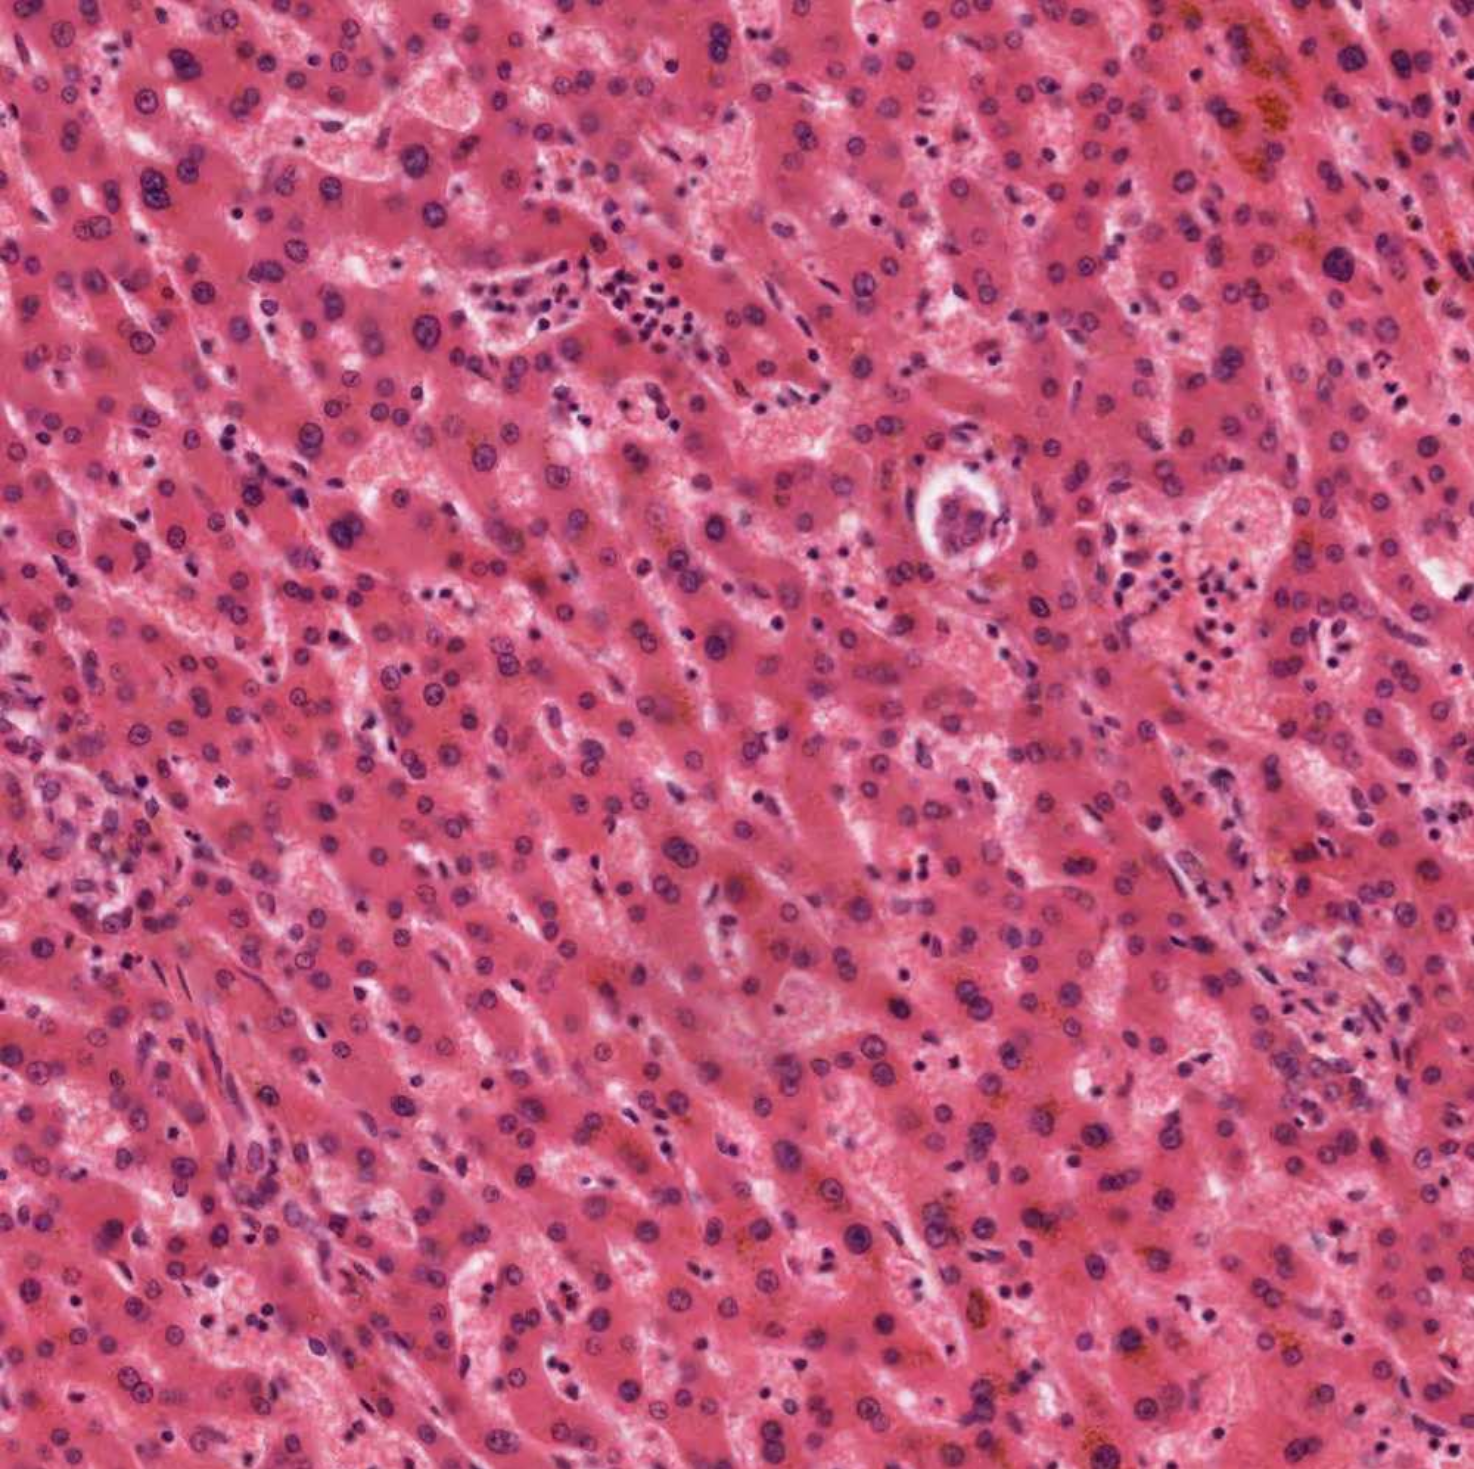
\includegraphics[width=\linewidth]{og.png} % ZMIANA: Upewnij się, że plik 'og.png' istnieje
        \caption{Oryginalny obraz}
        \label{fig:og}
    \end{minipage}
    \hfill
    \begin{minipage}{0.45\textwidth}
        \centering
        \includegraphics[width=\linewidth]{target.png} % ZMIANA: Upewnij się, że plik 'target.png' istnieje
        \caption{Obraz wzorcowy}
        \label{fig:target}
    \end{minipage}
\end{figure}

\begin{figure}[H]
    \centering
    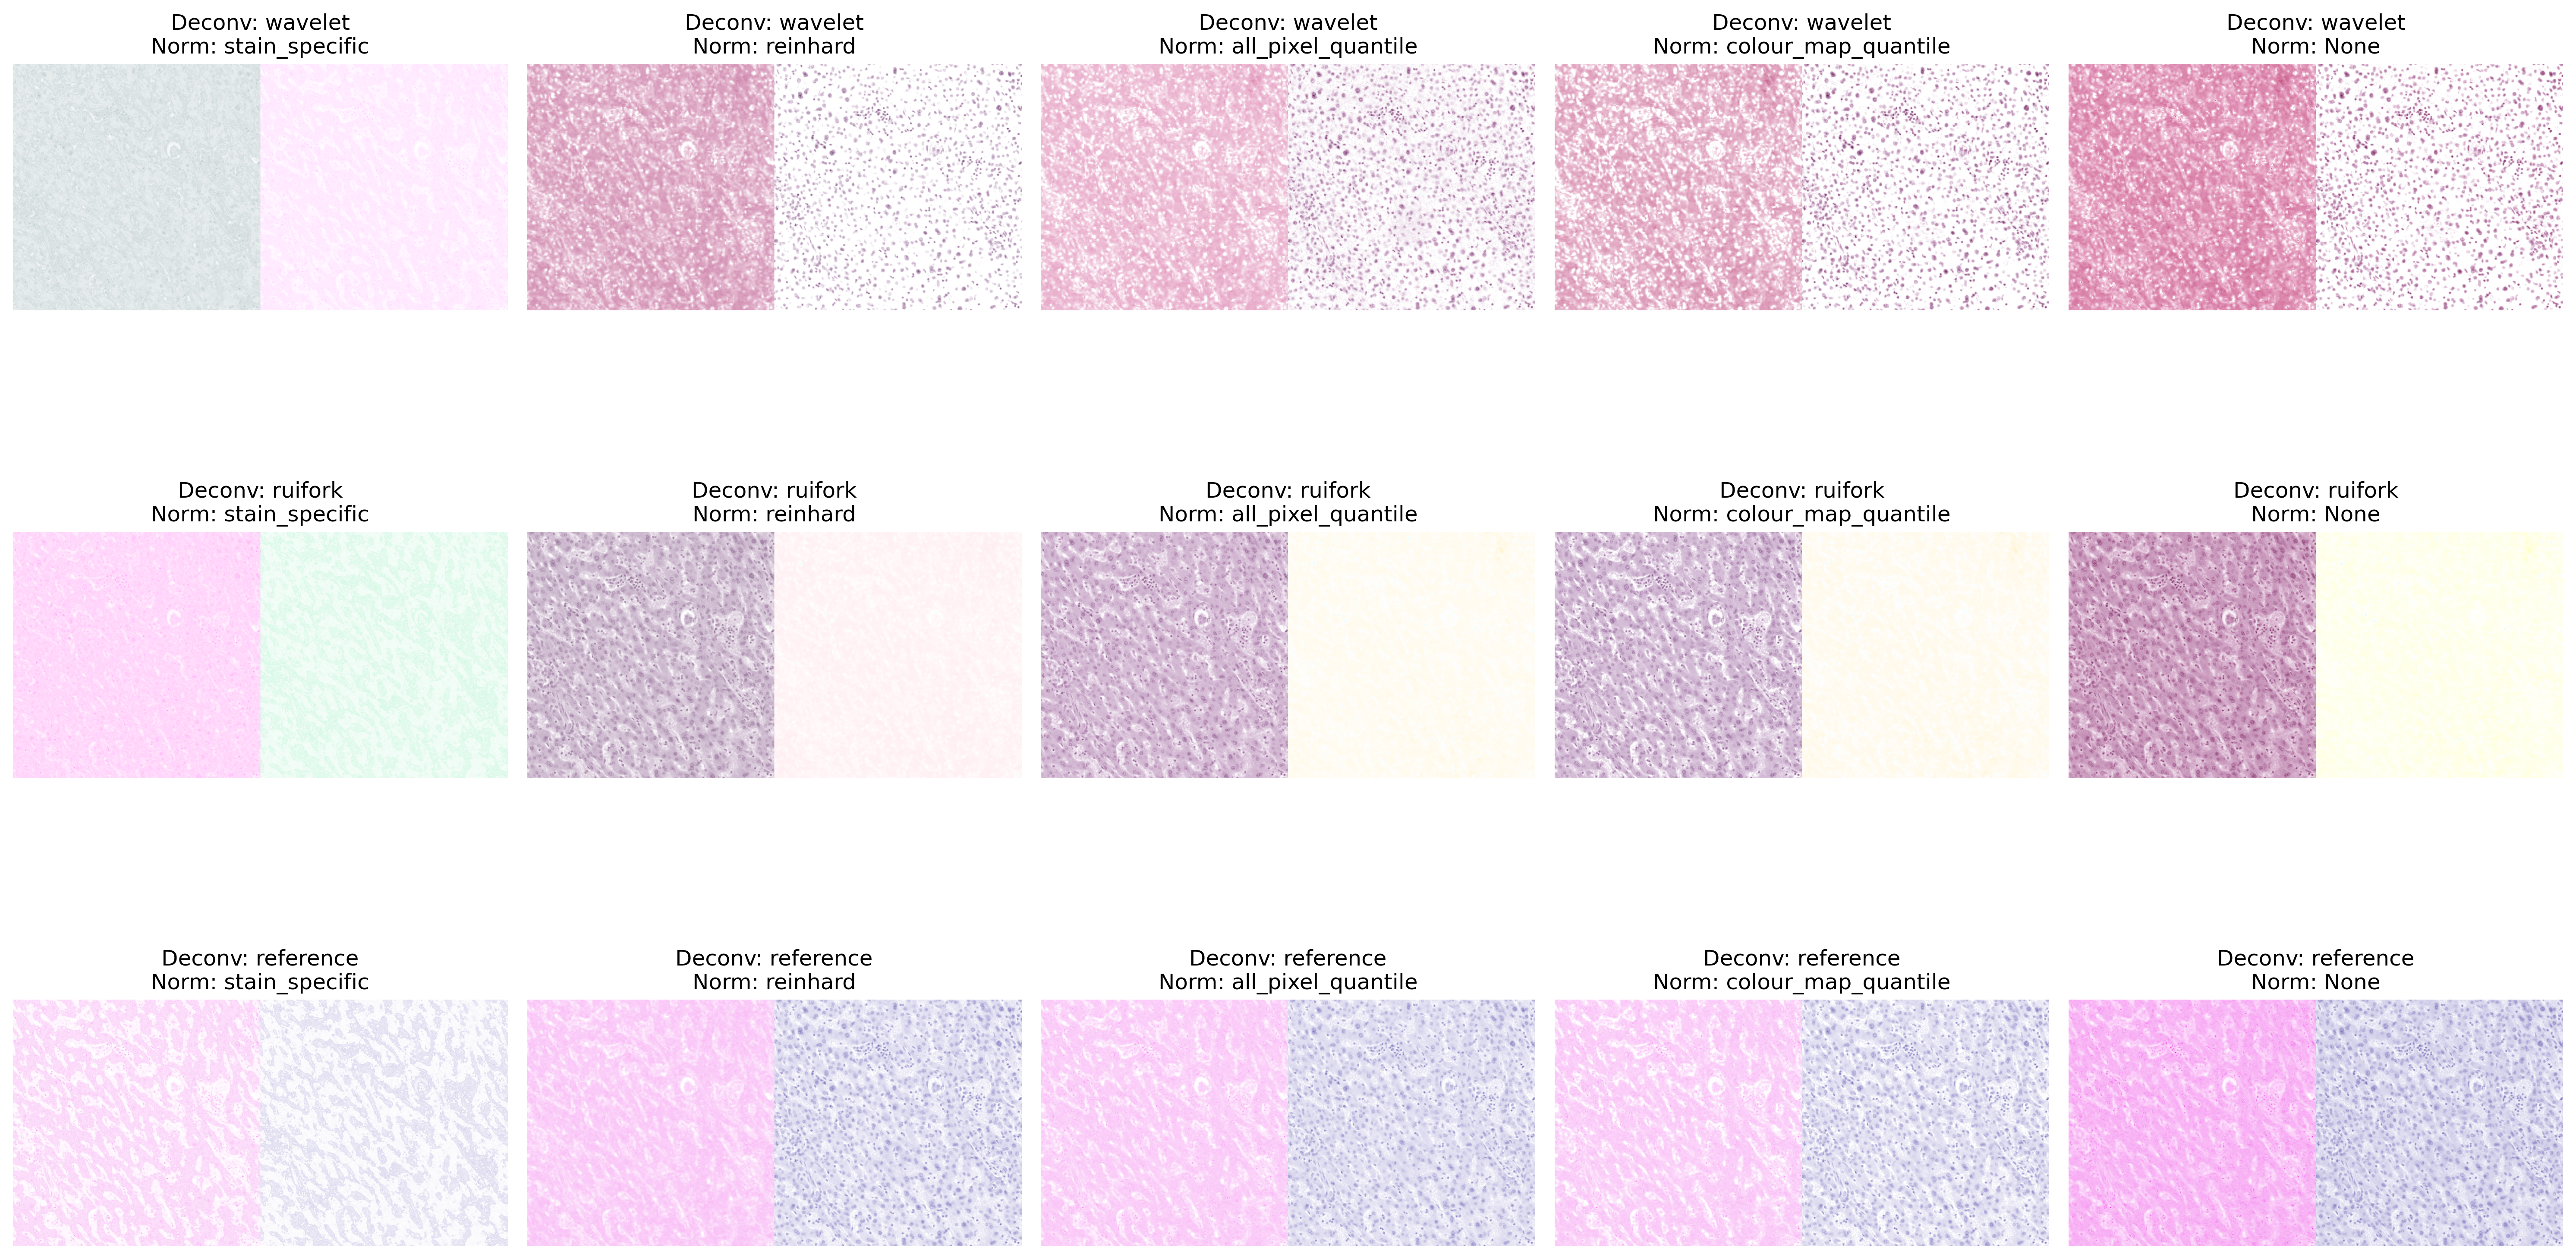
\includegraphics[width=0.9\linewidth]{methods_comparison.png} % ZMIANA: Upewnij się, że plik 'methods_comparison.png' istnieje
    \caption{Wizualne porównanie metod segmentacji barwników}
    \label{fig:methods_comparison}
\end{figure}

Klasyczne metody (Ruifrok, Reference) dają obrazy najbardziej zbliżone do standardowego barwienia H\&E, natomiast metoda falkowa (Wavelet + ICA) pozwala lepiej rozróżnić tekstury i struktury tkankowe, co może być korzystne przy automatycznej analizie obrazu, choć wizualnie odbiega od tradycyjnego wyglądu preparatu. Normalizacja (szczególnie Reinhard) zwiększa porównywalność próbek, zgodnie z teorią wyrównywania rozkładu kolorów.

\begin{figure}[H]
    \centering
    \includegraphics[width=0.75\linewidth]{mse.png} % ZMIANA: Upewnij się, że plik 'mse.png' istnieje
    \caption{MSE Rekonstrukcji}
    \label{fig:mse}
\end{figure}

Jeżeli spojrzymy na MSE rekonstrukcji, czyli średni błąd kwadratowy między oryginalnym obrazem a zrekonstruowanym, łatwo zauważyć, że najniższe wartości otrzymujemy dla kombinacji ruifork + none i wavelet + none.

\begin{figure}[H]
    \centering
    \includegraphics[width=0.75\linewidth]{wariancja.png} % ZMIANA: Upewnij się, że plik 'wariancja.png' istnieje
    \caption{Wariancja międzyklasowa}
    \label{fig:wariancja}
\end{figure}

Z drugiej strony, najlepszy wynik dla wariancji międzyklasowej otrzymujemy dla kombinacji wavelet + stain\_specific oraz lekko niższe reference + stain\_specific lub none. Czyli dla tych metod udaje się najlepiej rozdzielić poszczególne komponenty barwników.

\begin{figure}[H]
    \centering
    \includegraphics[width=0.75\linewidth]{korelacja.png} % ZMIANA: Upewnij się, że plik 'korelacja.png' istnieje
    \caption{Korelacja plam}
    \label{fig:korelacja}
\end{figure}

Jak spojrzymy na korelacje plam, czyli wskaźnik zgodności, między teoretycznym a uzyskanym rozkładem barwnika, można zauważyć, że ponownie zdecydowanie najlepsze wyniki otrzymujemy dla wavelet + stain\_specific oraz reference + stain\_specific, jednak tutaj reference + none ma jeden z najniższych wyników.

\begin{figure}[H]
    \centering
    \includegraphics[width=0.75\linewidth]{quantitative_timing_comparison.png} % ZMIANA: Upewnij się, że plik 'quantitative_timing_comparison.png' istnieje
    \caption{Porównanie czasowe}
    \label{fig:timing_comparison}
\end{figure}

\begin{table}[H]
\centering
\label{tab:czasy_przetwarzania}
\begin{tabular}{l r r r r}
\toprule
\textbf{Metoda} & \textbf{Średni czas [s]} & \textbf{Min [s]} & \textbf{Maks [s]} & \textbf{l. pomiarów} \\
\midrule
\multicolumn{5}{l}{\textbf{Czasy dekonwolucji}} \\
\midrule
wavelet     & 6.323 & 4.150 & 11.858 & 5 \\
ruifork     & 2.874 & 0.652 &  8.424 & 5 \\
reference  & 2.764 & 0.582 &  8.254 & 5 \\
\midrule
\multicolumn{5}{l}{\textbf{Czasy normalizacji}} \\
\midrule
stain\_specific       & 3.272 & 2.066 &  5.573 & 3 \\
reinhard             & 2.040 & 0.817 &  4.360 & 3 \\
all\_pixel\_quantile   & 3.317 & 2.104 &  5.675 & 3 \\
colour\_map\_quantile  & 9.512 & 8.254 & 11.858 & 3 \\
none                 & 1.795 & 0.582 &  4.150 & 3 \\
\bottomrule
\end{tabular}
\caption{Czasy przetwarzania metod dekonwolucji i normalizacji}
\end{table}
Na podstawie dokładnych pomiarów poszczególnych metod dekonwolucji oraz normalizacji, można zauważyć zdecydowanie dłuższy czas przetwarzanie dla metody wavelet oraz colour\_map\_quantile, co udowadnia nam również wykres.
\newpage
\begin{figure}
    \centering
    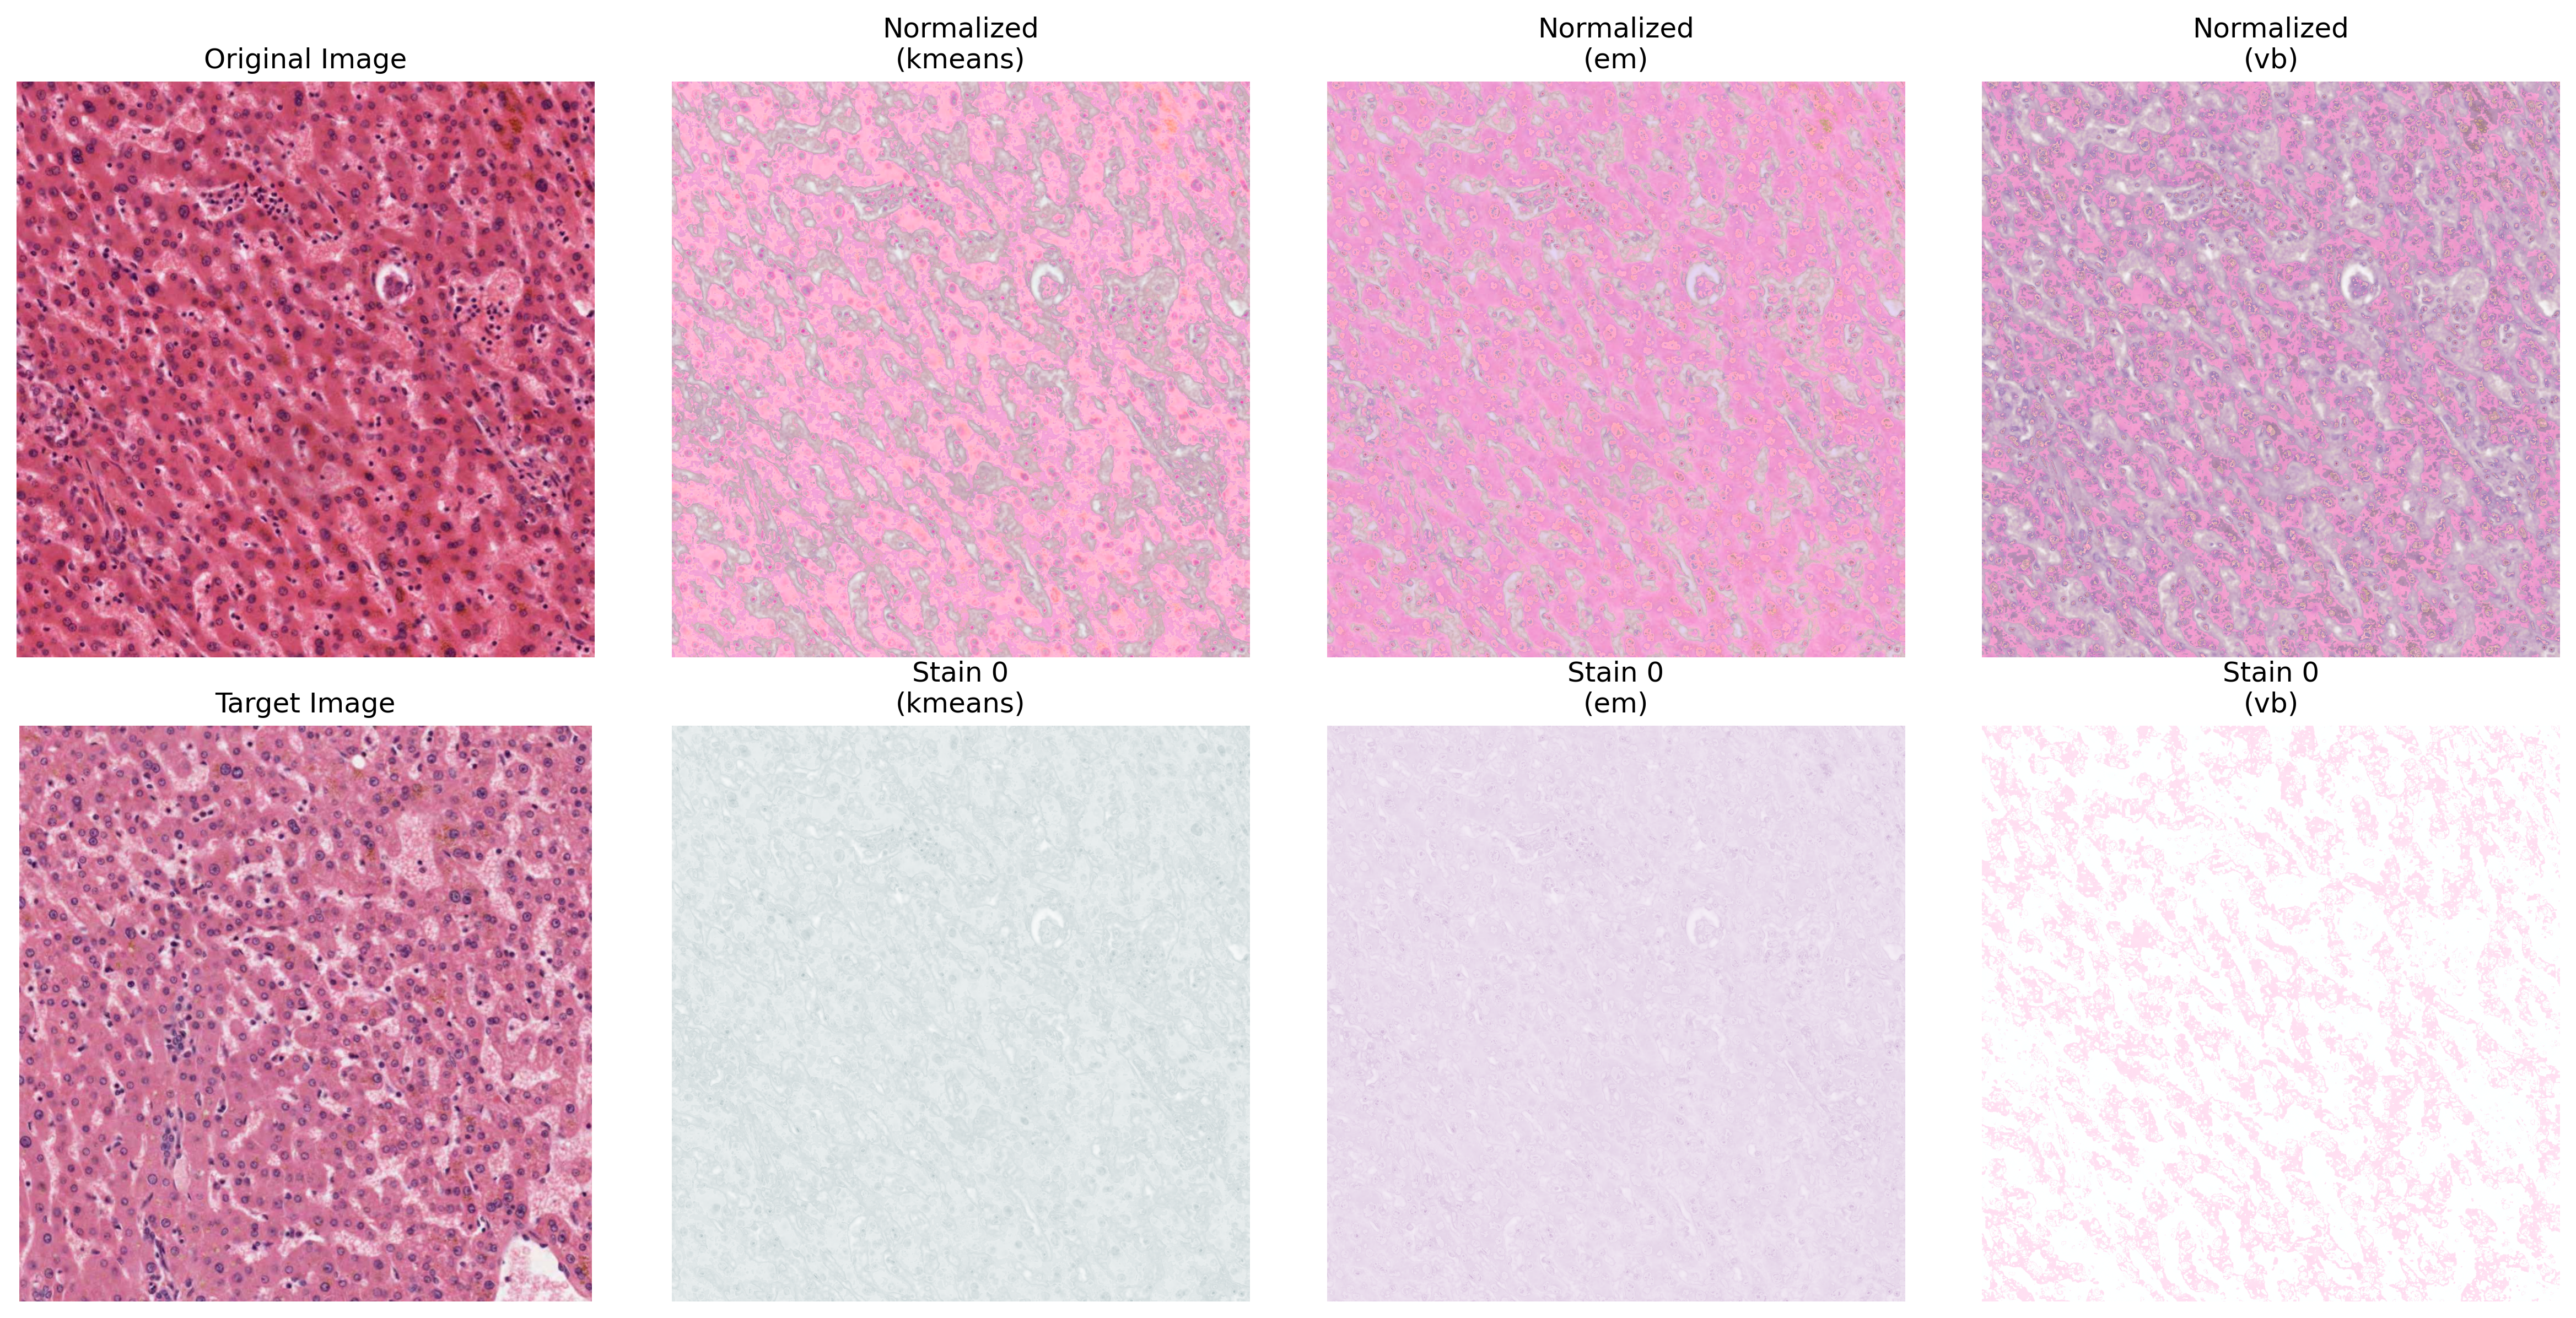
\includegraphics[width=0.75\linewidth]{clustering_comparison_wavelet_stain_specific.png}
    \caption{Wyniki różnych sposobów klastracji}
    \label{fig:placeholder}
\end{figure}

\begin{table}[h!]
\centering
\label{tab:podsumowanie}
\begin{tabular}{ll}
\toprule
\textbf{Metryka} & \textbf{Najlepsza metoda (wartość)} \\
\midrule
Separacja plam & \textbf{vb} (356.0462) \\
Korelacja plam & \textbf{em} (0.0369) \\
Błąd rekonstrukcji & \textbf{vb} (9612.4493) \\
Kontrast plamy 0 & \textbf{vb} (8.4842) \\
Kontrast plamy 1 & \textbf{vb} (14.1595) \\
Czas & \textbf{k-średnich} (29.82s) \\
\bottomrule
\end{tabular}
\caption{Najlepsze metody klastracji}
\end{table}

Na podstawie przeprowadzonych testów widać zdecydowaną przewage klastracji metodą GMM (vb), jednak ma ona również swoje wady, gdyż w testach czasowych wypada zdecydowanie najsłabiej, za to metoda k-średnich wypada zdecydowanie najlepiej czasowo, gdzie GMM potrzebowało aż 203.23s
\FloatBarrier

\section{Wnioski}

\begin{itemize}
\item \textbf{Metoda falkowa z ICA} okazała się najbardziej efektywna w separacji składników barwnikowych, osiągając najwyższe wartości wariancji międzyklasowej i korelacji plam, szczególnie w połączeniu z normalizacją stain-specific. Jest to preferowana metoda w zastosowaniach wymagających precyzyjnej analizy składników tkankowych.

\item \textbf{Normalizacja obrazów} znacząco wpływa na efektywność dekonwolucji. Normalizacja stain-specific dała najlepsze wyniki w poprawie separacji barwników, podczas gdy brak normalizacji (none) zapewnił najlepszą dokładność rekonstrukcji.

\item \textbf{Kompromis między dokładnością a czasem przetwarzania} jest wyraźnie widoczny. Metoda Wavelet + ICA, choć najwolniejsza, zapewnia najlepszą separację barwników, podczas gdy metoda Ruiforka oferuje najlepszy stosunek jakości do czasu przetwarzania.

\item \textbf{Metoda referencyjna} stanowi dobry kompromis między wszystkimi analizowanymi parametrami, oferując zrównoważone wyniki we wszystkich kategoriach. Jednak dla innego zestawu danych, zmiana wartości macierzy barwień może okazać się uciążliwa lub powodować niedokładne wyniki.
\end{itemize}

\begin{thebibliography}{9}
\bibitem{ruifrok}
Ruifrok, A. C., \& Johnston, D. A. (2001). Quantification of histochemical staining by color deconvolution. Analytical and quantitative cytology and histology, 23(4), 291-299.
\bibitem{wavelet}
Alsubaie et al. - 2016 - Stain deconvolution of histology images via independent component analysis in the wavelet domain
\bibitem{reinhard}
Magee et al. - Colour Normalisation in Digital Histopathology Images
\bibitem{normalization_comparison}
Hoffman et al. - 2014 - Comparison of normalization algorithms for cross-batch analysis
\end{thebibliography}

\end{document}